%%%%%%%%%%%%%%%%%%%%%%%%%%%%%%%%%%%%%%%%%
% University/School Laboratory Report
% LaTeX Template
% Version 3.1 (25/3/14)
%
% This template has been downloaded from:
% http://www.LaTeXTemplates.com
%
% Original author:
% Linux and Unix Users Group at Virginia Tech Wiki 
% (https://vtluug.org/wiki/Example_LaTeX_chem_lab_report)
%
% License:
% CC BY-NC-SA 3.0 (http://creativecommons.org/licenses/by-nc-sa/3.0/)
%
%%%%%%%%%%%%%%%%%%%%%%%%%%%%%%%%%%%%%%%%%

%----------------------------------------------------------------------------------------
%	PACKAGES AND DOCUMENT CONFIGURATIONS
%----------------------------------------------------------------------------------------

\documentclass{report}
\usepackage[utf8]{inputenc}
\usepackage{siunitx} % Provides the \SI{}{} and \si{} command for typesetting SI units
\usepackage{graphicx} % Required for the inclusion of images
\usepackage{caption}
\usepackage{natbib} % Required to change bibliography style to APA
\usepackage{amsmath} % Required for some math elements 
\usepackage{amssymb}
\usepackage{blindtext}
\usepackage{tikz}
\usetikzlibrary{matrix}
%\setlength\parindent{0pt} % Removes all indentation from paragraphs
\usepackage[framed]{matlab-prettifier}
\definecolor{mygreen}{RGB}{28,172,0} % color values Red, Green, Blue
\definecolor{mylilas}{RGB}{170,55,241}
\usepackage{listings}
\lstset{
	style=Matlab-editor,
	basicstyle         = \fontsize{8}{11}\ttfamily,
	numberstyle       =\fontsize{8}{11}\ttfamily,
	%backgroundcolor=\color{gray},
	%mlshowsectionrules = true,
	rangeprefix        = \%\ 
}

\renewcommand{\labelenumi}{\alph{enumi}.} % Make numbering in the enumerate environment by letter rather than number (e.g. section 6)

%\usepackage{times} % Uncomment to use the Times New Roman font
%----------------------------------------------------------------------------------------
%	TITLE PAGE
%----------------------------------------------------------------------------------------
% Title Page
\title{TIC}
\author{Mauricio Caceres}
\date{18 décembre 2016}

%----------------------------------------------------------------------------------------
%	DOCUMENT INFORMATION
%----------------------------------------------------------------------------------------

\begin{document}
\begin{titlepage}
	\centering
	\vfill
{\bfseries\huge Technologie de l'information et codage}
	\vfill
	{\bfseries\LARGE
		TP:\\
		Codage de source et optimisation de la \\capacité du canal
		\\
		\vskip2cm

		Master SISEA\\
	
	}
	\vfill
	18 décembre 2016
	\vfill
	{\large Mauricio Caceres } \hfill  {\large Enseignant : Claude Cariou}
	\vfill
	
\includegraphics[width=9cm]{rennes} % also works with logo.pdf    
	\vfill
	
\includegraphics[width=6cm]{enssat} % also works with logo.pdf
	\vfill
	\vfill
\end{titlepage}
\tableofcontents

%\begin{center}
%\begin{tabular}{l r}
%Date Performed: & January 1, 2012 \\ % Date the experiment was performed
%Partners: & James Smith \\ % Partner names
%& Mary Smith \\
%Instructor: & Professor Smith % Instructor/supervisor
%\end{tabular}
%\end{center}


% If you wish to include an abstract, uncomment the lines below
% \begin{abstract}
% Abstract text
% \end{abstract}

%----------------------------------------------------------------------------------------
%	SECTION 1
%----------------------------------------------------------------------------------------
\chapter{Introduction}
\section{Objectif}

L’objectif de ce TP est de vérifier expérimentalement la théorie de Shannon en utilisant les
outils de la théorie de l’information (entropie, information mutuelle). Plus précisément, il
s’agira d’optimiser le couple source-canal : considérant un canal binaire non symétrique.\\ Il
faudra déterminer \textbf{(théoriquement et expérimentalement) }les conditions optimales d’utilisation
de ce canal, c’est-à-dire trouver la distribution de probabilité des symboles d’entrée maximisant
l’information mutuelle entre l’entrée et la sortie.




\subsection{Definitions}
\label{definitions}
\begin{description}
\item[Canal]
Un canal discret sans mémoire est un modèle
statistique comportant une entrée X (variable aléatoire) et une sortie Y
(variable aléatoire), qui est une version bruitée de X.

La source émet un symbole issu de l'alphabet par exemple A
\begin{equation}\label{key}
A=\{x_0,x_1,...,x_{j-1}\}
\end{equation}
La sortie du canal discret sans mémoire est un symbole issu de l'alphabet
que nous appellerons B
\begin{equation}\label{key}
B=\{y_0,y_1,...,y_{i-1}\}
\end{equation}
Chaque un des éléments de l'ensemblez
\item[Canal binaire non symétrique]
Le canal est caractérisé par ses probabilités de transition. Dans un canal no symétrique 
les probabilités de transition ne sont pas égales.


\begin{figure}[h]
	\centering
	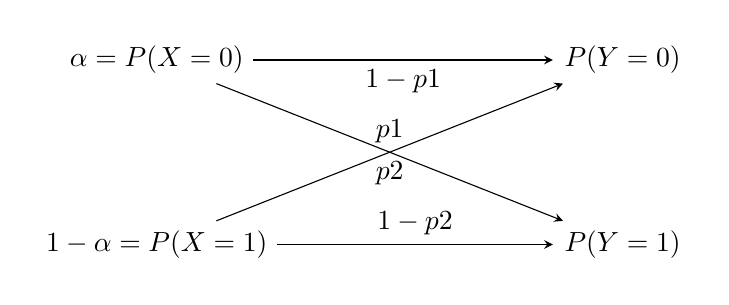
\begin{tikzpicture}
	\matrix (m) [matrix of math nodes,row sep=5em,column sep=10em,minimum width=5em]
	{
		\alpha = P(X = 0)  & P(Y = 0)\\
		1-\alpha = P(X = 1)  & P(Y = 1) \\};
	\path[-stealth]
	(m-1-1) edge node [below] {$1-p1$} (m-1-2)
	(m-2-1) edge node [below] {$p2$} (m-1-2)
	(m-1-1) edge node [above] {$p1$} (m-2-2)
	(m-2-1) edge node [above] {$1-p2$} (m-2-2);
	
	\end{tikzpicture}
	\label{img:schema_transition}
	\caption{schèma du transition du canal}
\end{figure}

\item[Information mutuelle]
L'information gagnée sur l'observation d'un évènement est à cause de que existe 
une certaine quantité de surprise un niveuau d'incertitude. On utilise cette concept
et la notion d'entropie pour comprendre comment est définie l'information mutuelle.\\
\begin{figure}[h]
	\centering
	\captionsetup{justification=centering}
	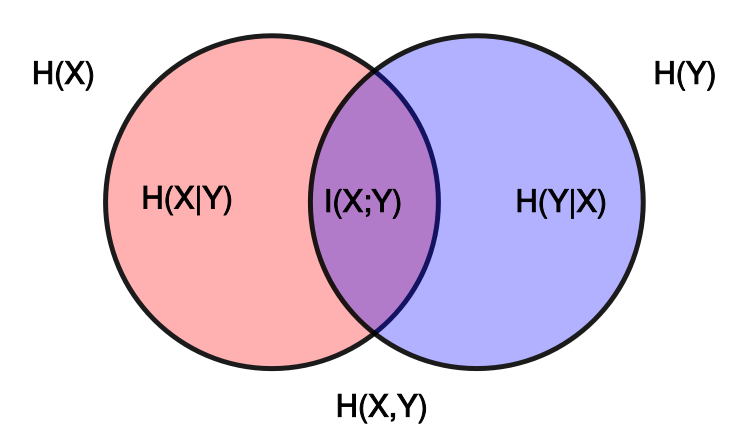
\includegraphics[width=0.5\linewidth]{info}
	\caption{Entropies individuelles (H(X),H(Y)),\\ jointes (H(X,Y)), d'une couple (X, Y),\\ avec l'information mutuelle I(X; Y).}
	\label{fig:info}
\end{figure}%todo reviser
$H(X)$ est l’incertitude sur l’entrée avant l’observation de la
sortie. $H(X | Y)$ est l’incertitude sur l’entrée après l’observation de
la sortie. Si même $H(X) – H(X | Y)$ représente l’incertitude sur l’entrée
résolue par l’observation de la sortie, ce qui est défini comme information mutuelle.


\item[Capacité du canal]%todo reviser 
la capacité d’un canal discret sans mémoire
est le maximum de l’information mutuelle I(A, B) moyenne
obtenu pour l’ensemble des symboles émis, la
maximisation étant opérée sur toutes les distributions a
priori possibles $\{p ( x j ) \}$ sur A.
\begin{equation}\label{capaciteCanal}
C = maxI(A,B)
\end{equation}
Sous les cointraintes 
\begin{equation}\label{key}
 p ( x_j ) \geq 0 ; \forall j \qquad \sum_{j=0}^{J-1}p ( x_j )=1
\end{equation}
\end{description} 



%----------------------------------------------------------------------------------------
%	SECTION 2
%----------------------------------------------------------------------------------------
\chapter{Implémentation en MATLAB{\small \circledR}}

\section{Génération d'une séquence binaire}
Pour effectuer la simulation du canal nous avons besoin d'avoir une séquence aléatoire de un alphabet binaire.
Dans la Fig. \ref{img:schema_transition} on voit bien que la probabilité de que $P(X=0)$ est défini comme un 
$\alpha$ qui sera notre paramètre. On pourra générer un séquence de tout zéros pour un $\alpha = 1$ et uns séquence de toutes un pour $\alpha = 0$
Dans le code \ref{code_sequence} nous avons utilisé la fonction \texttt{randsrc} ou on désigne 
l'alphabet à utiliser et la probabilité de chaque éléments.

\begin{lstlisting}[caption={Code générateur de séquence bynaire aléatoire},label=code_sequence]
help randsrc
%[...] 
% If ALPHABET is a two-row matrix, the first row defines the
% Matrix  possible outputs (as above).  The second row of ALPHABET
% specifies the probability for each corresponding element.  The
% elements of the second row must sum to one.
%[...] 
alphabet = [0 1 ; alpha 1-alpha];
S=randsrc(1,N,alphabet);
\end{lstlisting}

\section{Simulation du canal asymétrique}
En suivant le schèma de la Fig.\ref{img:schema_transition_2} on a pu coder la simulation comme est 
montre dans le code \ref{code_simulation}.\\
Sachant que le canal est caractérise pour les probabilités de transition $P(Y = 1|X = 0)=p1$ $ P(Y = 0|X = 1)=p2 $ l'idée de l'implementation est évaluer a chaque fois le contenu de $X$ la séquence aléatoire d'entrée et selon si sa 
valeur est 1 ou 0 on va générer un séquence aléatoire (d'un élément) avec un probabilité pour 0 et 1 donnée pour soit $p1$ ou bien $p2$. Il peut avoir de problèmes si on désigne de manière
incorrecte les probabilités.

\begin{figure}[h]
	\centering
	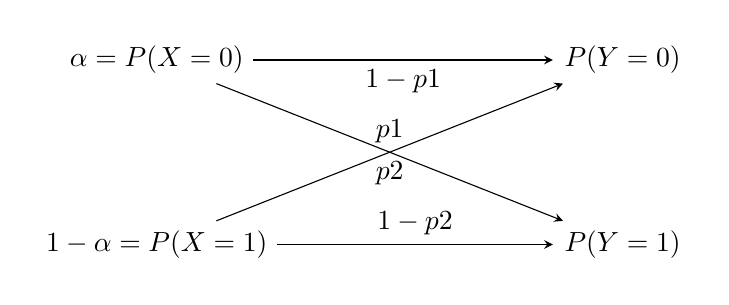
\begin{tikzpicture}
	\matrix (m) [matrix of math nodes,row sep=5em,column sep=10em,minimum width=5em]
	{
		\alpha = P(X = 0)  & P(Y = 0)\\
		1-\alpha = P(X = 1)  & P(Y = 1) \\};
	\path[-stealth]
	(m-1-1) edge node [below] {$1-p1$} (m-1-2)
	(m-2-1) edge node [below] {$p2$} (m-1-2)
	(m-1-1) edge node [above] {$p1$} (m-2-2)
	(m-2-1) edge node [above] {$1-p2$} (m-2-2);
	
	\end{tikzpicture}
	\caption{canal BNS}
	\label{img:schema_transition_2}
\end{figure}

\begin{lstlisting}[caption={Code pour les probabilite de transition $P(Y = 1|X = 0)=p1$ $ P(Y = 0|X = 1)=p2 $},label=code_simulation]
%% version en utilisant meme function seqbinaire
     for i = 1:length(X)
         if(X(i) == 0) %en sachant X=0
                Y(i) =  seqbinaire(1,1-p1); % proba de element 0 de l'alphabet donc 1-p1
         else             %en sachant X=1
                Y(i) =  seqbinaire(1,p2);
         end  
     end
 
\end{lstlisting}

La version implementé dans le code \ref{code_simulation} a pris beacoup de temps de simulation. Pour 
soigner cette problème l'utilisation du code \ref{code_simulation_2} qui fait pas à pas l'affectation
des valeurs selon les probabilités données. Le temps de simulation a été réduit considérablement

%todo acomodar el codigo
\begin{lstlisting}[caption={Code },label=code_simulation_2]
    for i = 1:length(X)
if(X(i) == 0) %en sachant X=0
if rand()< p1 
Y(i) = 1;  % p(Y=1|X=0)=p1
else              
Y(i) = 0; %sinon Y = 0 avec proba = 1-p1
end
else             %en sachant X=1
if rand()< p2
Y(i) = 0; % p(Y=0|X=1)=p2
else
Y(i) = 1; %sinon Y = 0 avec proba = 1-p2
end      
end
end
\end{lstlisting}

\section{Estimation de l'information mutuelle}
On connait la définition de l'information mutuelle
\begin{equation}\label{eq:I}
I(X,Y) = H(Y) - H(Y|X);
\end{equation}
La stratégie est calculer les entropies séparément. D'abord l'entropie de la sortie $Y$
\begin{equation}\label{eq:II}
H(Y) = -P(Y=0)log(P(Y=0))-P(Y=1)log(P(Y=1))
\end{equation}
Et ensuite l'entropie conditionnelle
\begin{eqnarray}\label{key}
H(Y|X)= (-P(Y=0|X=0)log2(P(Y=0|X=0))-\nonumber\\P(Y=1|X=0)log2(P(Y=1|X=0)))P(X=0)\nonumber\\ +(-P(Y=0|X=1)log2(P(Y=0|X=1))-\nonumber\\P(Y=1|X=1)*log2(P(Y=1|X=1)))(P=X1);\nonumber\\
\label{eq:III}
\end{eqnarray}
On voit bien que il faut avoir la valeur de tous les probabilités pour effecteur le calcul. Donc on va les estimer dans la section suivante (\ref{sec:estimation}).

\subsection{Estimation de probabilités sur l'entrée et la sortie}
\label{sec:estimation}
En utilisant la équation suivante on peut estimer la valeur des probabilités. Ces valeurs de 
probabilité seront utilisés pour le calcul de l'information mutuelle expérimentale
\begin{equation}\label{eq:probconde}
P(Y=0) \approx 1/N \sum_{n=1}^{N}  \mathbf{1}_{y_n=0}
\end{equation}

Pour notre cas on fait la somme des occurrences de numéro 1 et ensuite on calcule la probabilité 
complémentaire.
\begin{equation}\label{eq:probcond}
P(Y=1) \approx 1/N \sum_{n=1}^{N}  \mathbf{1}_{y_n=1}\qquad P(Y=0) = 1 - P(Y=1)
\end{equation}

\begin{equation}\label{eq:probcondee}
P(X=1) \approx 1/N \sum_{n=1}^{N}  \mathbf{1}_{x_n=1}\qquad P(X=0) = 1 - P(X=1)
\end{equation}

En utilisant la fonction \texttt{find} de Matlab on peut trouver les éléments non nuls 
dedans un vecteur. Dans le code \ref{code_conditional} on voit l'implémentation d'une fonction
qui fait tout le travail.
\vfill
\begin{lstlisting}[caption={Code },label=code_conditional]
function [IXY]=info_mutuelle(X,Y) 
%  Fonction pour  Estimation   I(X,Y) = H(Y) - H(Y|X);
%% Variables
N = length(X);
NY = length(Y);

%% Estimation de P(X = 0) et P(X = 1)
NXones = length(find(X));
NXzeros = N - NXones ;
PX1 = NXones/N; %find cherche les elements non nuls
PX0 = 1 - PX1;

%% Estimation de P(Y = 0) et P(Y = 1)
NYones =  length(find(Y));
NYzeros =  N - NYones;
PY1 = NYones/NY;
PY0 = 1 - PY1;
...
...
\end{lstlisting}

\subsection{Estimation de probabilités conditionnelles}
Avec la même notion de probabilités estime on calcule les probabilites conditionneles.
\begin{equation}\label{key}
P(Y=1|X=0) \approx 1/N_{x_n=0} \sum_{n=1}^{N}  \mathbf{1}_{y_n=1,x_n=0} 
\end{equation}

\begin{equation}\label{key}
P(Y=1|X=1) \approx 1/N_{x_n=1} \sum_{n=1}^{N}  \mathbf{1}_{y_n=1,x_n=1} 
\end{equation}

\begin{lstlisting}[caption={Code },label=code_]

for i = 1:N
%% Estimation de P(Y = 0|X = 0) et P(Y = 0|X = 1) 
if Y(i)==0 && X(i)== 0
		PY0X0 =  PY0X0 +1;  %% count P(Y = 0|X = 0)
	elseif Y(i)==0 && X(i)==1
		PY0X1 = PY0X1+1;    % count P(Y = 0|X = 1                  
	%% Estimation de P(Y = 1X = 0) et P(Y = 1|X = 1) 
	elseif Y(i)==1 && X(i) == 0  
		PY1X0 =  PY1X0 +1;   %count for P(Y = 1X = 0)
	elseif Y(i)==1 && X(i) == 1
		PY1X1 =PY1X1 + 1;   %count for P(Y = 1|X = 1) 
	end
end
%utiliser bayes
PY1X1 = PY1X1/NXones;
PY1X0 = PY1X0/NXzeros;
PY0X1 = PY0X1/NXones; 
PY0X0 = PY0X0/NXzeros;
...
...
\end{lstlisting}

En ayant maintenant tous les valeurs on pourra effecteur le calcul avec les équations 
,\ref{eq:II},\ref{eq:III}. On peut passer a l'étape suivante.
%\begin{equation}\label{key}
%H(Y) = -P(Y=0)log(P(Y=0))-P(Y=1)log(P(Y=1))
%\end{equation}
%
%\begin{eqnarray}\label{key}
%H(Y|X)= (-P(Y=0|X=0)log2(P(Y=0|X=0))-\nonumber\\P(Y=1|X=0)log2(P(Y=1|X=0)))P(X=0)\nonumber\\ +(-P(Y=0|X=1)log2(P(Y=0|X=1))-\nonumber\\P(Y=1|X=1)*log2(P(Y=1|X=1)))(P=X1);\nonumber\\
%\end{eqnarray}
%
%\begin{equation}\label{key}
%I(X,Y) = H(Y) - H(Y|X);
%\end{equation}



%----------------------------------------------------------------------------------------
%	SECTION 3
%----------------------------------------------------------------------------------------
\chapter{Analyses et conclusions}
\section{Courbes et données obtenues}
La trace de la fonction $I(X,Y)=f(\alpha)$ est donnée dans la Fig. \ref{fig:superposition}
Avec les paramètres données pour $p1 = 0.1$ et $p2 = 0.2$ et une discrétisation avec 200 points sur l'échelle d'alpha.\\
Dans cette figure on verra aussi que les deux courbes se superposes assez bien.
\begin{figure}[h]
	\centering
	\captionsetup{justification=centering}
	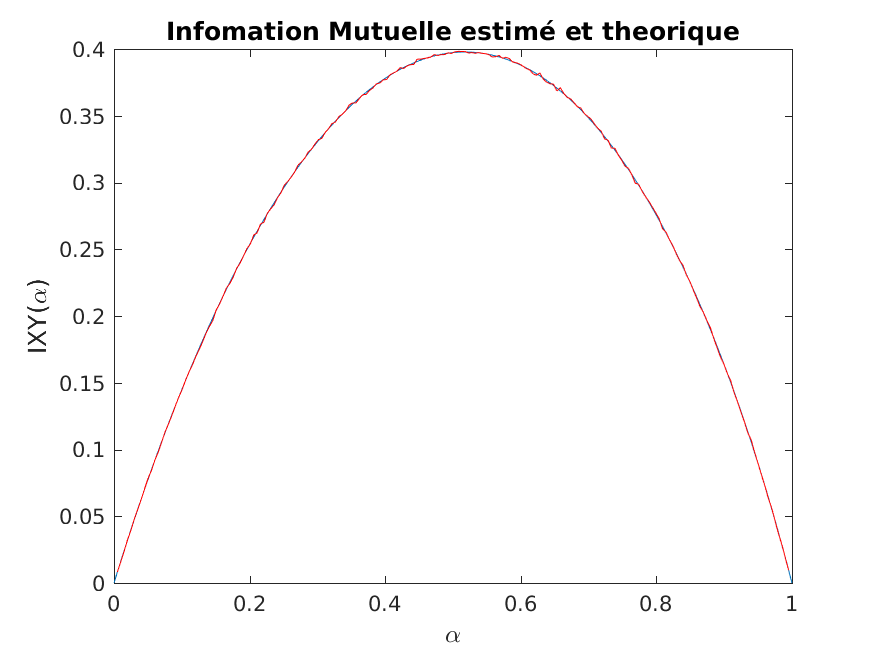
\includegraphics[width=0.7\linewidth]{../canal1}
	%todo caption
	\caption{}
	\label{fig:superposition}
\end{figure}
Le début et fin de la coube en 0 et un bonne signal de que elle est correcte. \\
Dans la figure \ref{fig:errorsuposition} la courbe montre l'erreur avec un facteur d'échelle de 30 (pour le voir mieux, parce que l'erreur est petit) entre chaque courbe la théorique et l'expérimentale
\begin{figure}[h]
	\centering
	\captionsetup{justification=centering}
	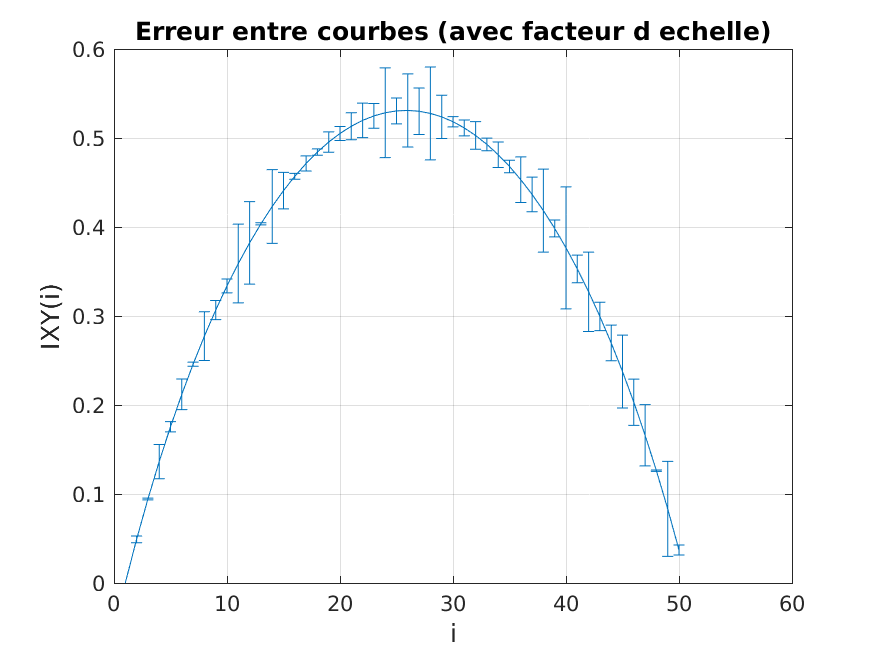
\includegraphics[width=0.5\linewidth]{../canal2}
	%todo caption
	\caption{}
	\label{fig:errorsuposition}
\end{figure}
L'effet de que les courbes sont presque identiques est que on a une séquence X d'entrée très longue ($N=10e6$) et cela fait que la estimation soit très précise
\begin{figure}[h]
	\centering
	\captionsetup{justification=centering}
	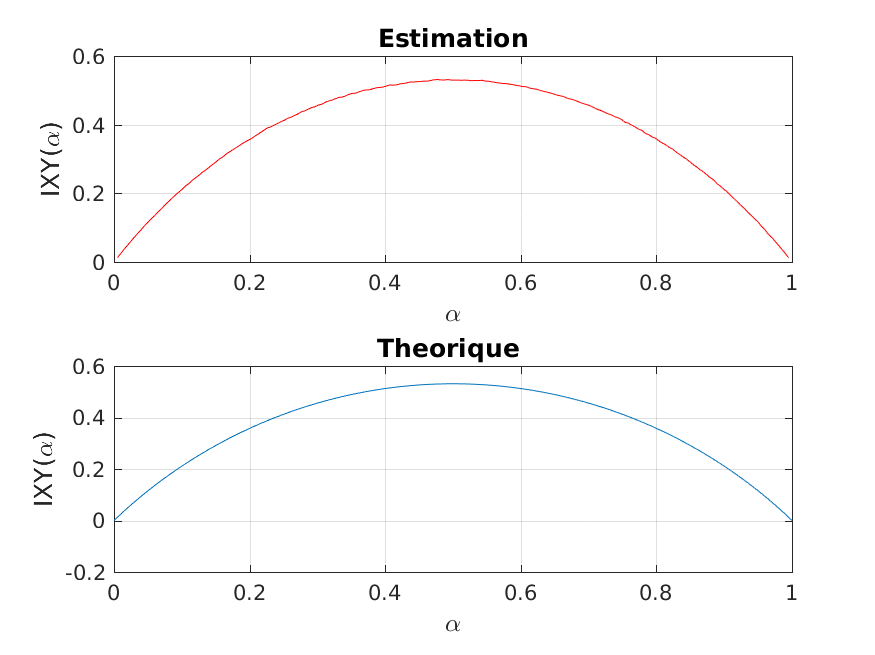
\includegraphics[width=0.6\linewidth]{../canal3}
	%todo caption
	\caption{}
	\label{fig:}
\end{figure}


\section{Conclusion}


\begin{figure}[h]
	\centering
	\captionsetup{justification=centering}
	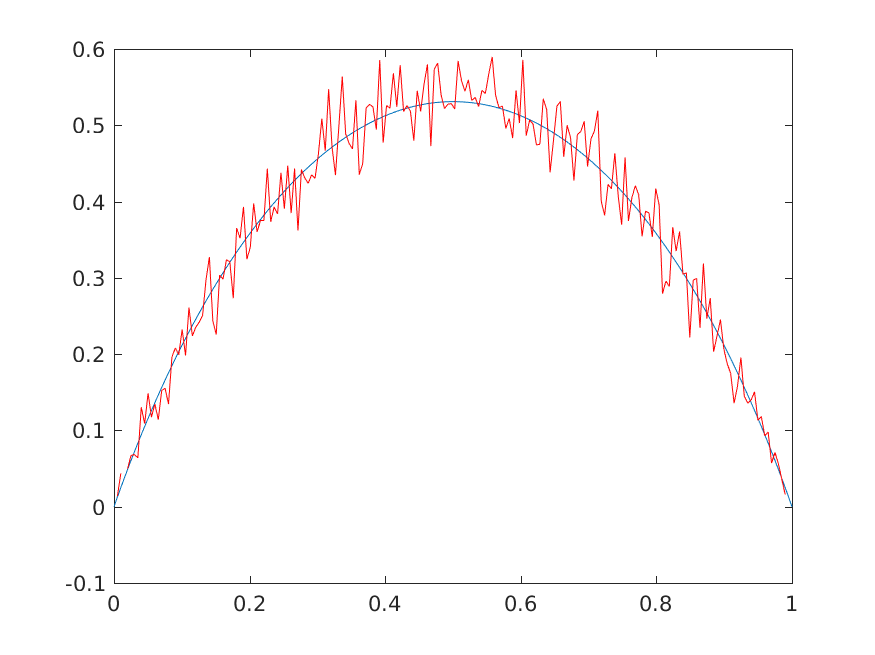
\includegraphics[width=0.7\linewidth]{../canal21}
	%todo caption
	\caption{}
	\label{fig:}
\end{figure}


\begin{figure}[h]
	\centering
	\captionsetup{justification=centering}
	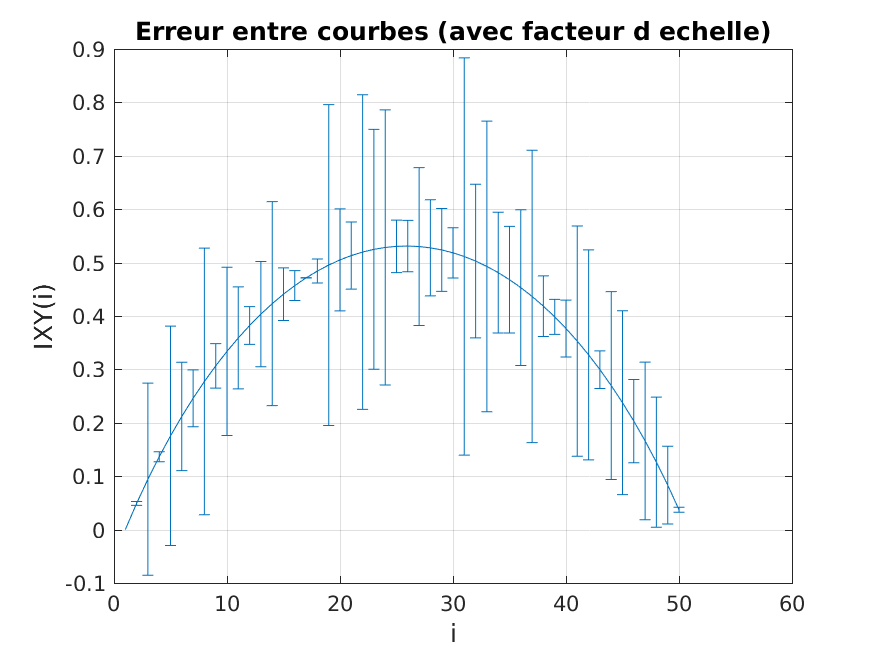
\includegraphics[width=0.7\linewidth]{../canal22}
	%todo caption
	\caption{}
	\label{fig:}
\end{figure}

\begin{figure}[h]
	\centering
	\captionsetup{justification=centering}
	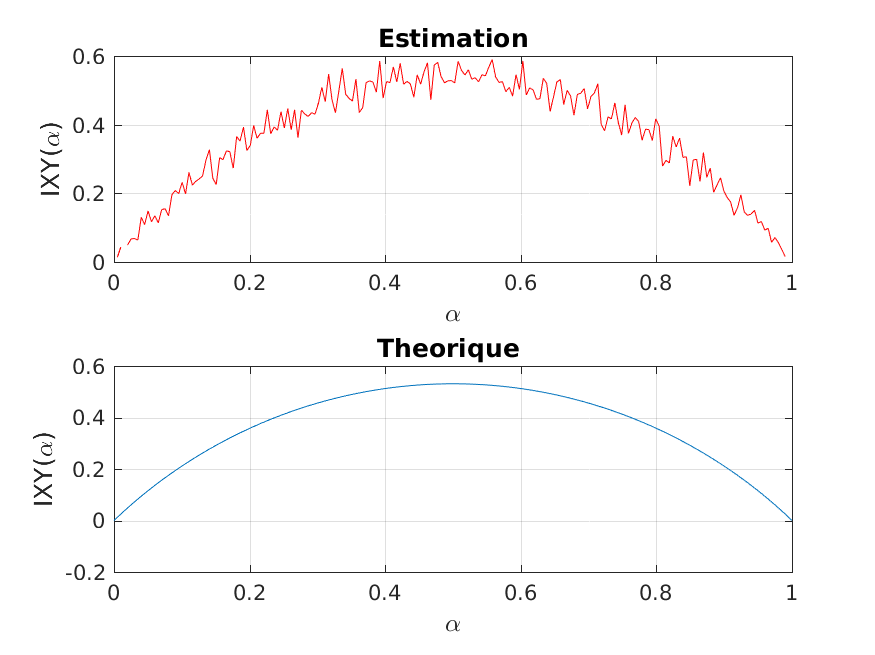
\includegraphics[width=0.7\linewidth]{../canal23}
	%todo caption
	\caption{}
	\label{fig:}
\end{figure}
Une autre méthode de simulation en utilisant des masques binaire a été implémente qui améliore beaucoup
la vitesse de la simulation, mais malheureusement ne donne pas de bonnes valeur parce que elle est mal conçu. Un tâche pour améliorer le code pourra être bien implémenter cette solution.

%----------------------------------------------------------------------------------------
%	FIN
%----------------------------------------------------------------------------------------



\end{document}























